\section{Implementation and Results}
The proposed Tsception model was trained on data of 15 subjects. The 10-fold cross-validation method was carried out on the data. One fold was used for testing, and the remaining 9 folds were used for training. The model was trained for 100 epochs with a batch size of 64. The model was trained using the Adam optimizer with a learning rate of $0.0001$ and a weight decay of $0.0001$. The ratio $\alpha$ used for the kernel window size was $0.125$, $0.25$, $0.5$. The number of hidden nodes in LSTM was kept as 128. The model was evaluated for two dimensions, Arousal' and Valence'. The model was evaluated using two important metrics: validation accuracy and F1 score.
The following training loss and validation loss vs epochs plots were obtained for the first 8 subjects without LSTM for a randomly picked trial.
\begin{figure}[h]
    \centering
    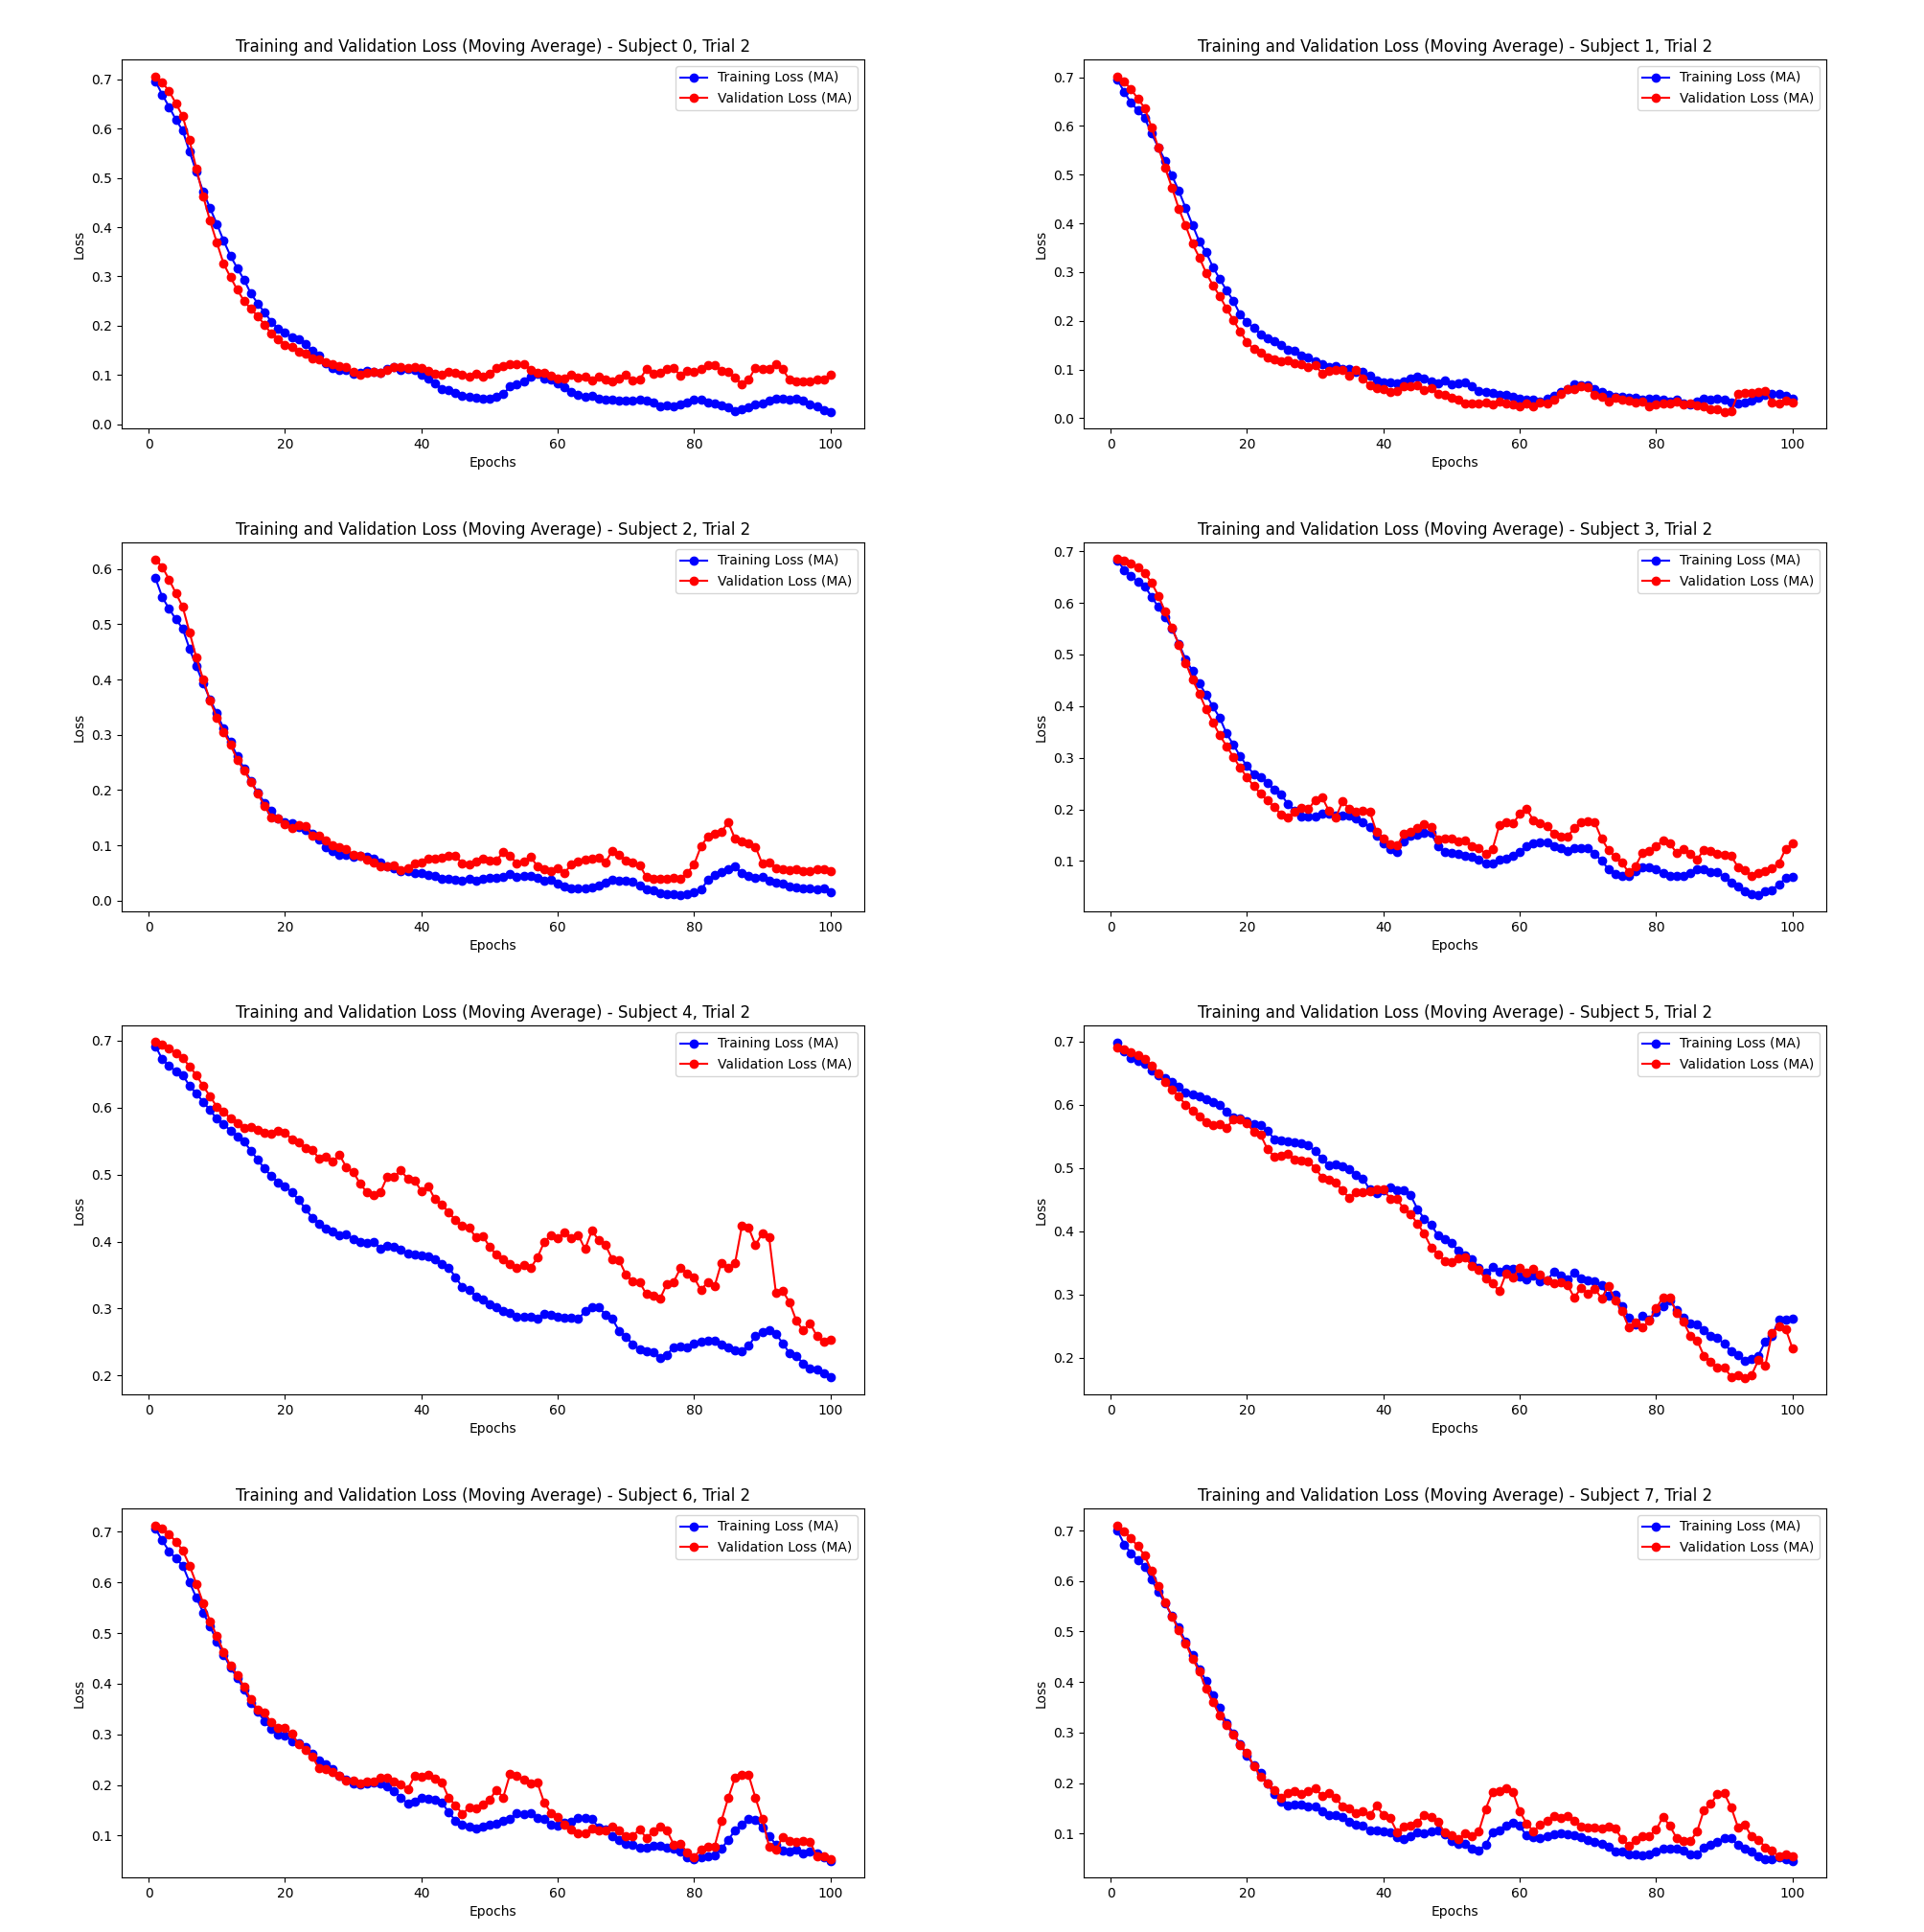
\includegraphics[width=0.5\textwidth, height = 10cm]{combined.png} % Adjust the path and the scaling factor
    \caption{Loss vs epochs without LSTM} % Caption for the image
    \label{loss vs epoch without LSTM} % Label for referencing the image elsewhere in the text
\end{figure}

The following training loss and validation loss vs epochs plots were obtained for the first 8 subjects without LSTM for a randomly picked trial.

\begin{figure}[h]
    \centering
    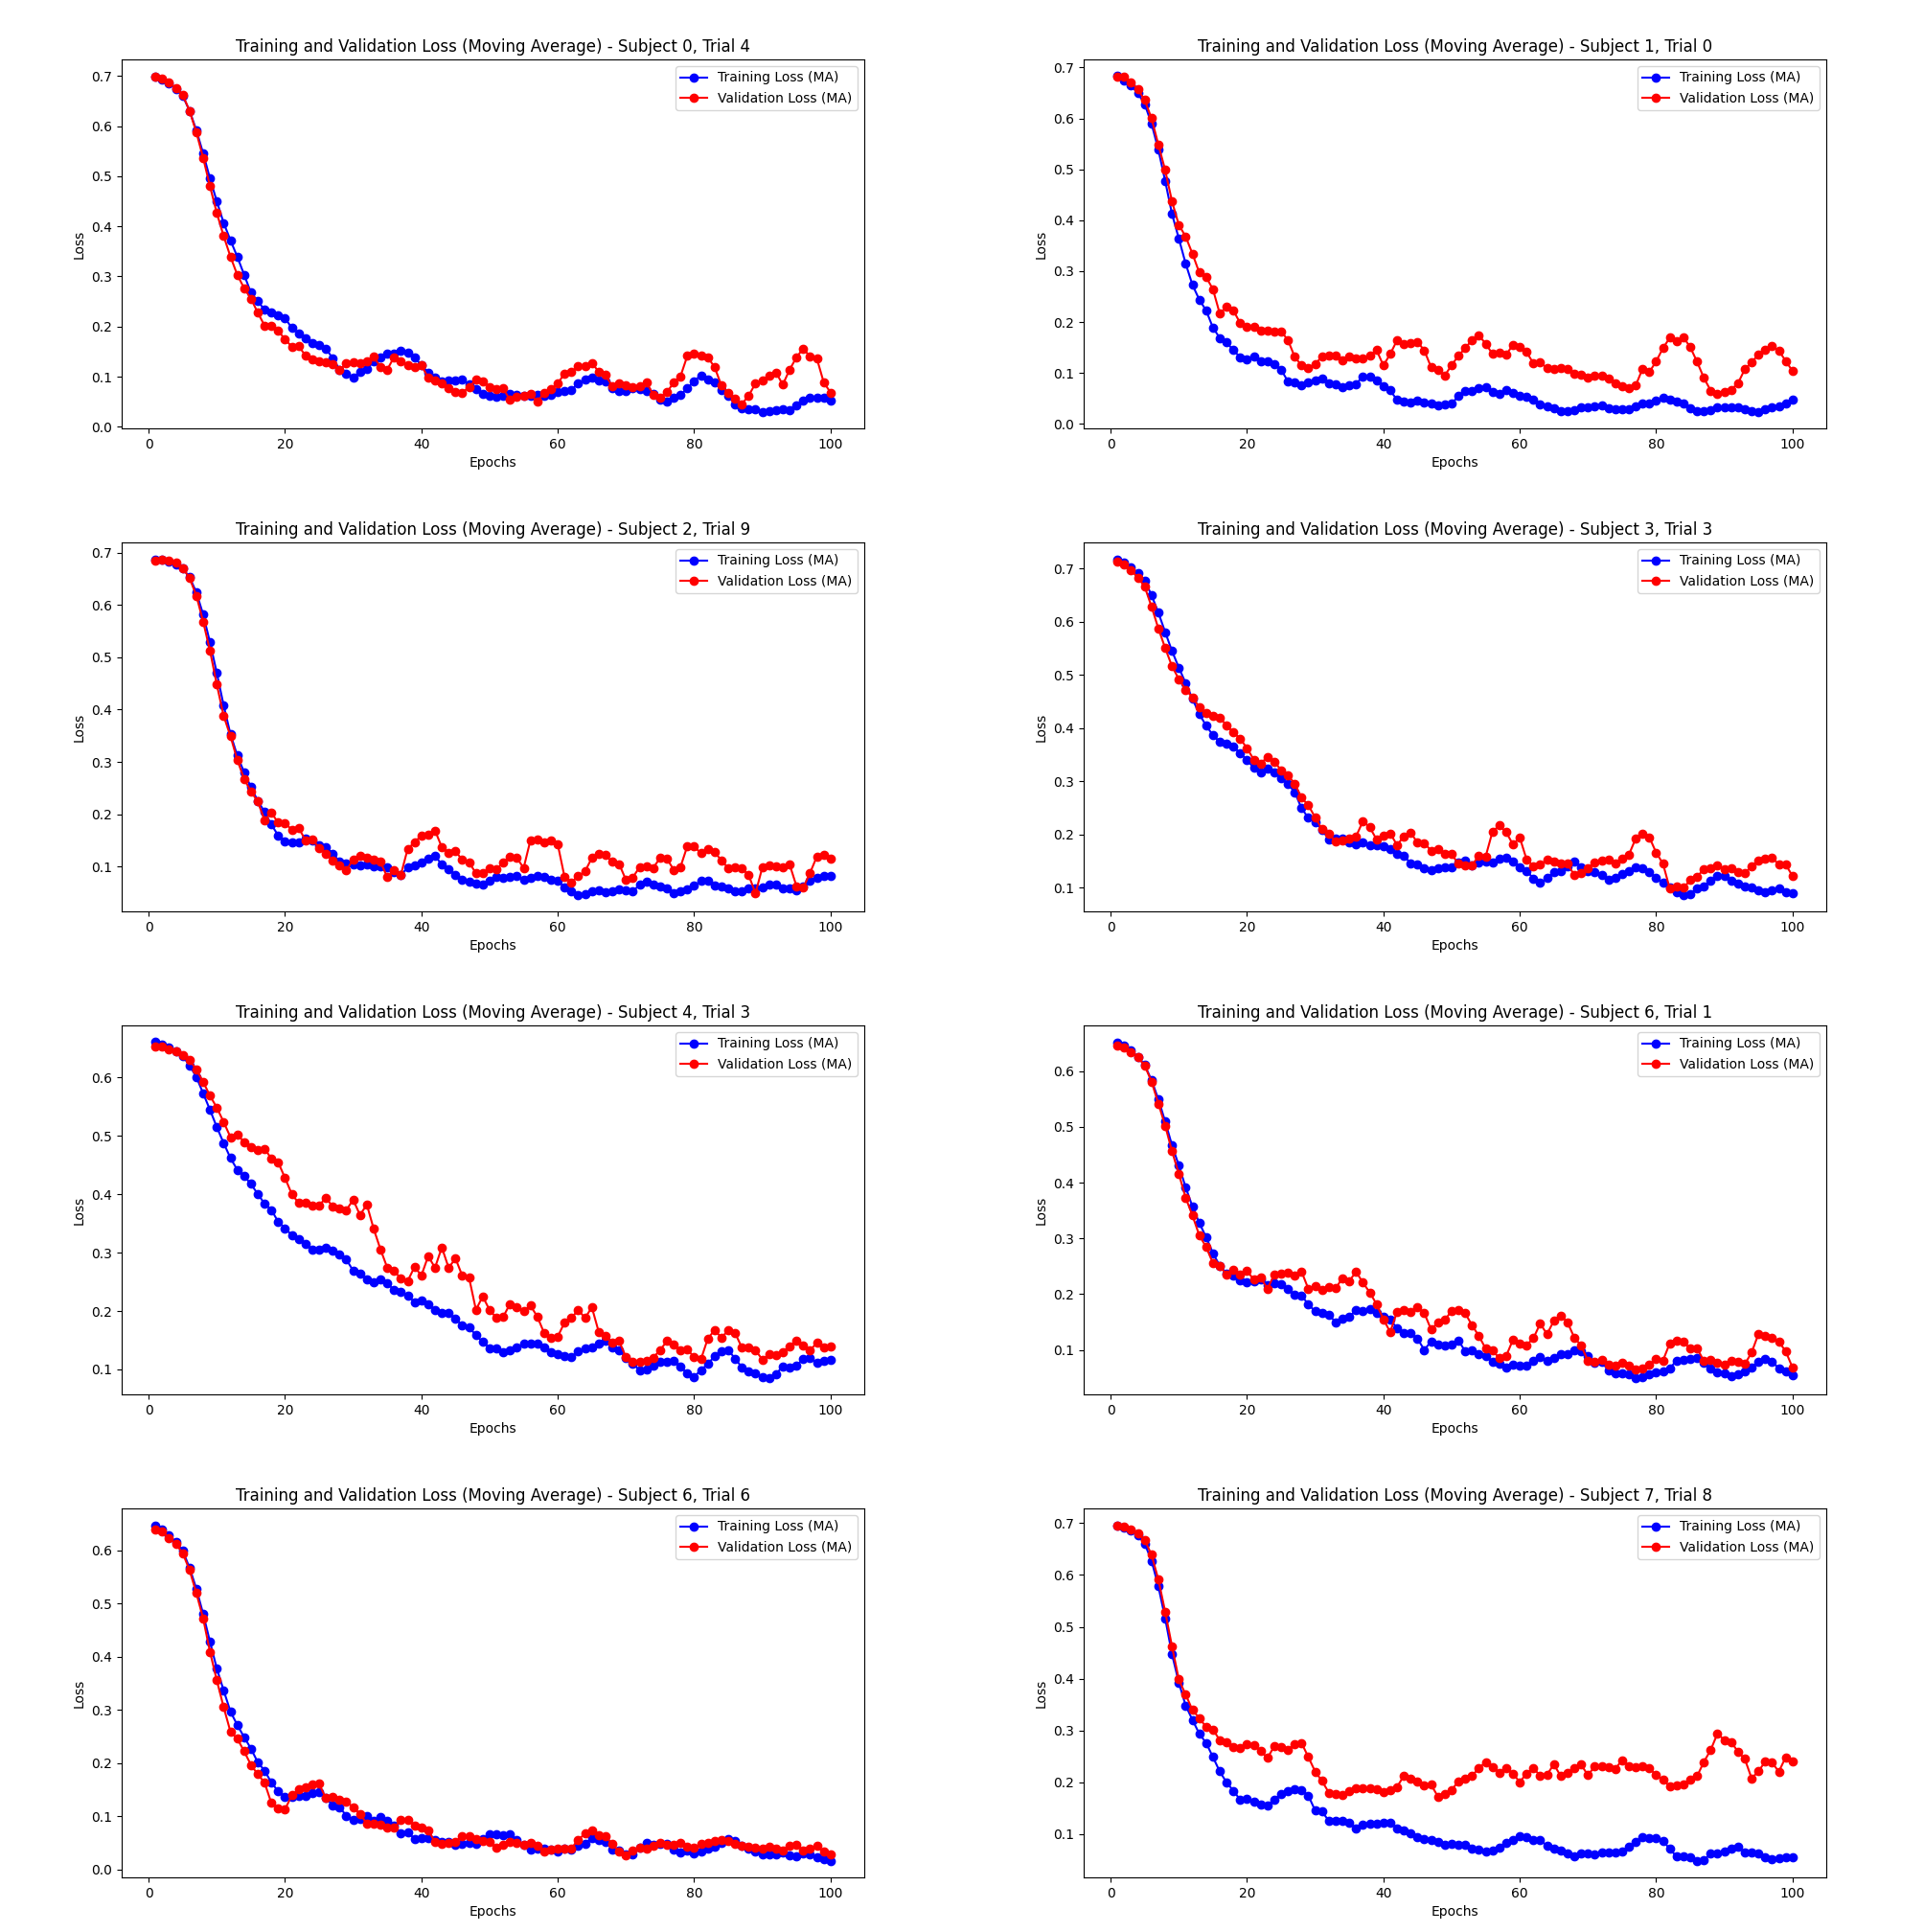
\includegraphics[width=0.5\textwidth, height =10cm]{new_combined.png} % Adjust the path and the scaling factor
    \caption{Loss vs epochs with LSTM} % Caption for the image
    \label{loss vs epoch with LSTM} % Label for referencing the image elsewhere in the text
\end{figure}

With LSTM, the loss decreases more steeply in the initial epochs compared to those without LSTMS. LSTMS contribute to faster convergence. Fluctuautions in the validation loss are lesser with using LSTM showing more robustness and generalizability of the model. Also the final loss values at the end of 100 epochs is lower for the Tsception model with LSTM than without.

The proposed model have an accuracy and F1 score higher than the original model for both the dimensions arousal and valence. The accuracy for arousal and valence show improvemnet with LSTM with accuracies of $0.9325$ and $0.926$ respectively as compared to older Tsception model with accuracies of $0.9162$ and $0.9156$ for arousal and valence dimensions respectively. ALong with this the F1 scores also show a significant improvement with scores of $0.944$ and $0.938$ with LSTM as compared to $0.923$ and $0.9185$ for older model.

The proposed model shows an overall improvement of $1.77$\% and $0.5$\% in accuracy for arousal and valence respectively. The F1 score also shows an improvement of $2.2$\% and $1.9$\% for arousal and valence dimensions respectively.
\begin{table}[ht]
    \centering
    \begin{tabular}{lcr} % alignment for each column (left, center, right)
    \toprule
    metric & with LSTM & Without LSTM  \\
    \midrule
    Arousal & 0.9325 & 0.9162 \\
    Valence & 0.9205 & 0.9156 \\
    \bottomrule
    \end{tabular}
    \caption{Accuracy comparison}
    \label{tab:example}
\end{table}
\begin{table}[ht]
    \centering
    \begin{tabular}{lcr} % alignment for each column (left, center, right)
    \toprule
    metric & with LSTM & Without LSTM  \\
    \midrule
    Arousal & 0.944 & 0.923 \\
    Valence & 0.938 & 0.9185 \\
    \bottomrule
    \end{tabular}
    \caption{F1 scores comparison}
    \label{tab:example}
\end{table}
    
    


